% =====================================================================
% Figure 1 — Landauer-gated execution schematic (TikZ)
%
% Standalone document: compile as-is in Overleaf (or pdflatex) to preview.
% To use in the paper, copy the \begin{tikzpicture}...\end{tikzpicture}
% block into a figure environment; the required \usetikzlibrary lines go
% in the preamble.
%
% Faithful to Section 2.1 (the three equations) and Section 2.2 (energy
% regimes). Palette matches the data figures (Wong colorblind-safe).
% =====================================================================
\documentclass[border=6pt]{standalone}
\usepackage{amsmath}
\usepackage{amssymb}
\usepackage{tikz}
\usetikzlibrary{shapes.geometric, arrows.meta, positioning, backgrounds, fit, calc}

% ---- Wong colorblind-safe palette (matches figs 2-6) ----
\definecolor{golblue}{HTML}{0072B2}   % execute / go
\definecolor{bbverm}{HTML}{D55E00}    % hold / blocked
\definecolor{neut}{HTML}{555555}      % guides
\definecolor{dngreen}{HTML}{009E73}   % energy

\begin{document}
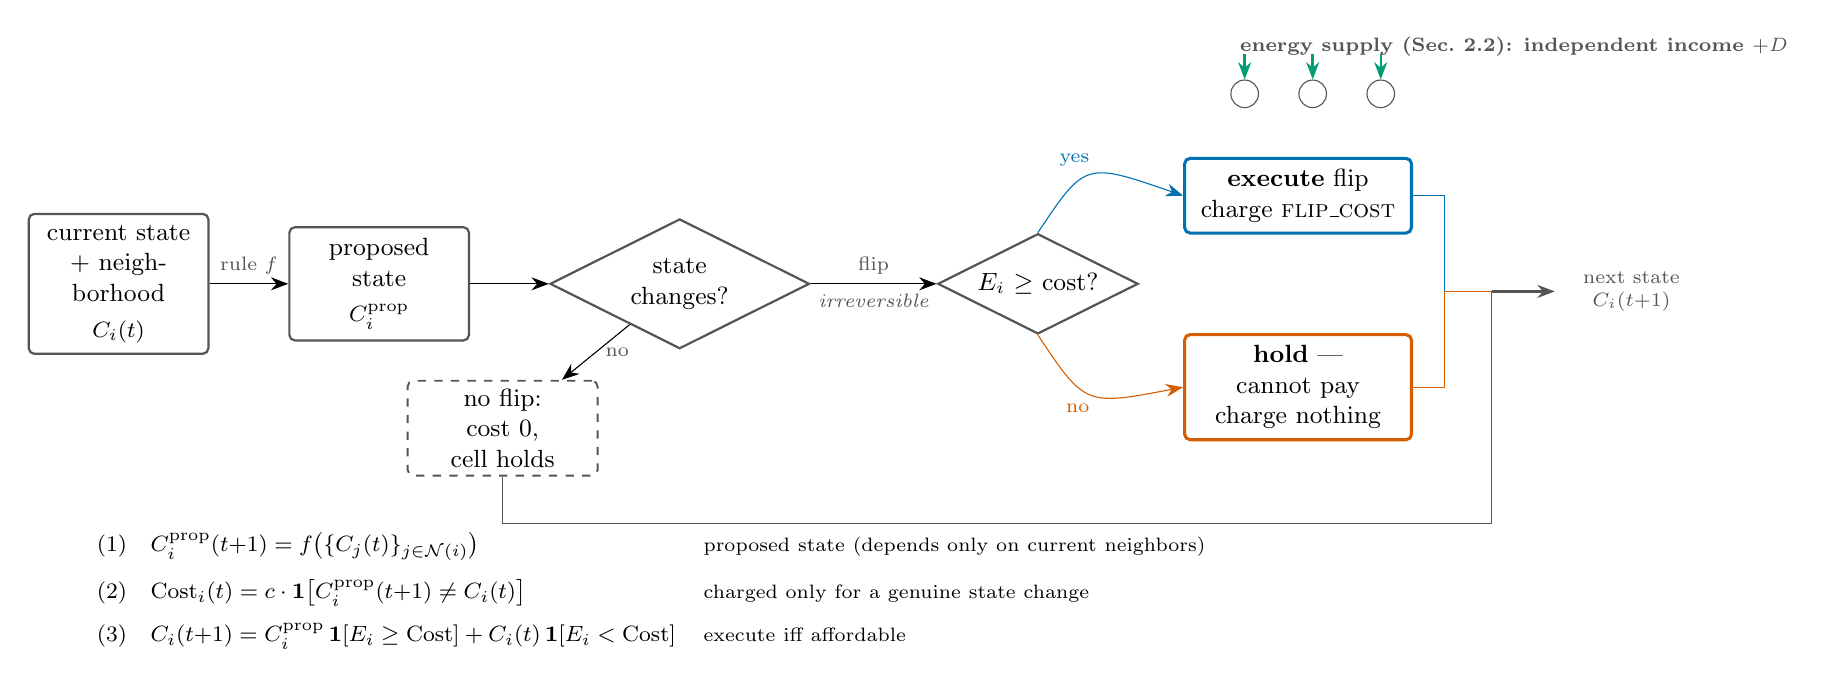
\begin{tikzpicture}[
  font=\small,
  >={Stealth[length=2.2mm]},
  every node/.style={align=center},
  proc/.style={rectangle, rounded corners=2pt, draw=neut, line width=0.8pt,
               inner sep=4pt, minimum height=9mm, text width=20mm},
  go/.style={rectangle, rounded corners=2pt, draw=golblue, line width=1.1pt,
             inner sep=4pt, minimum height=9mm, text width=26mm},
  hold/.style={rectangle, rounded corners=2pt, draw=bbverm, line width=1.1pt,
               inner sep=4pt, minimum height=9mm, text width=26mm},
  dec/.style={diamond, aspect=2, draw=neut, line width=0.8pt, inner sep=1pt,
              minimum width=22mm, minimum height=11mm, text width=18mm},
  freebox/.style={rectangle, rounded corners=2pt, draw=neut, dashed,
                  line width=0.7pt, inner sep=3pt, text width=22mm, minimum height=8mm},
  lab/.style={neut, font=\scriptsize},
]

% ---------- main left-to-right flow ----------
\node[proc] (cur) {current state\\ + neighborhood\\[2pt]\footnotesize $C_i(t)$};
\node[proc, right=10mm of cur] (prop) {proposed\\ state\\[2pt]\footnotesize $C_i^{\text{prop}}$};
\node[dec, right=10mm of prop] (d1) {state\\ changes?};
\node[dec, right=16mm of d1] (d2) {$E_i \ge$ cost?};

% execute / hold outcomes (stacked at right)
\node[go,  above right=3mm and 12mm of d2] (exec) {\textbf{execute} flip\\ charge \textsc{flip\_cost}};
\node[hold, below right=3mm and 12mm of d2] (holdb) {\textbf{hold} — cannot pay\\ charge nothing};

% "no change" free path (drops below-left of d1, clear of the equations)
\node[freebox, below left=8mm and 2mm of d1] (free) {no flip:\\ cost $0$, cell holds};

% ---------- arrows ----------
\draw[->] (cur) -- node[lab,above]{rule $f$} (prop);
\draw[->] (prop) -- (d1);
\draw[->] (d1) -- node[lab,above]{flip} node[lab,below]{\itshape irreversible} (d2);
\draw[->] (d1) -- node[lab,right]{no} (free);
\draw[->, golblue] (d2.north) .. controls +(0.6,0.9) .. (exec.west)
      node[lab, pos=0.55, above left=-1pt]{\color{golblue}yes};
\draw[->, bbverm] (d2.south) .. controls +(0.6,-0.9) .. (holdb.west)
      node[lab, pos=0.55, below left=-1pt]{\color{bbverm}no};

% converge to next-state (right edge)
% All three outcome paths (execute, hold, no-flip) MERGE at a bus point,
% then a single arrow drives forward -> next state (nothing points backward).
\coordinate (bus) at ($(exec.east)!0.5!(holdb.east) + (10mm,0)$);
\node[right=8mm of bus, text width=17mm, lab, anchor=west] (next) {next state\\ $C_i(t{+}1)$};
% execute and hold feed into the vertical bus (no arrowheads — they merge)
\draw[golblue] (exec.east) -- ++(4mm,0) |- (bus);
\draw[bbverm] (holdb.east) -- ++(4mm,0) |- (bus);
% single forward arrow from the bus into next state
\draw[->, neut, line width=1.0pt] (bus) -- (next.west);
% free path routes DOWN, around underneath, and up into the SAME bus (merge, no backward head)
\draw[neut] (free.south) -- ++(0,-6mm) -| (bus);

% ---------- the three equations (sidebar, fully below the flow) ----------
\node[below=22mm of d1, text width=150mm, align=left, font=\footnotesize] (eqs) {
  \setlength{\arraycolsep}{2pt}
  $\begin{aligned}
    \text{(1)}\quad & C_i^{\text{prop}}(t{+}1) = f\big(\{C_j(t)\}_{j\in\mathcal{N}(i)}\big)
       && \text{\scriptsize proposed state (depends only on current neighbors)}\\[3pt]
    \text{(2)}\quad & \text{Cost}_i(t) = c\cdot \mathbf{1}\!\left[C_i^{\text{prop}}(t{+}1)\neq C_i(t)\right]
       && \text{\scriptsize charged only for a genuine state change}\\[3pt]
    \text{(3)}\quad & C_i(t{+}1) = C_i^{\text{prop}}\,\mathbf{1}\!\left[E_i\ge\text{Cost}\right]
       + C_i(t)\,\mathbf{1}\!\left[E_i<\text{Cost}\right]
       && \text{\scriptsize execute iff affordable}
  \end{aligned}$
};

% ---------- energy-supply inset (small, top-right corner) ----------
\begin{scope}[shift={($(exec.north west)+(6mm,14mm)$)}, font=\scriptsize]
  \node[lab, anchor=west] (etitle) at (0,0) {\textbf{energy supply (Sec.\ 2.2): independent income $+D$}};
  % independent income — three cells each with their own inflow arrow
  \node[circle, draw=neut, minimum size=3.5mm, below=6mm of etitle.west, anchor=west] (c1) {};
  \node[circle, draw=neut, minimum size=3.5mm, right=5mm of c1] (c2) {};
  \node[circle, draw=neut, minimum size=3.5mm, right=5mm of c2] (c3) {};
  \foreach \c in {c1,c2,c3} \draw[->, dngreen, line width=0.9pt] ($(\c)+(0,5mm)$) -- (\c);
\end{scope}

\end{tikzpicture}
\end{document}
